%%%%%%%%%%%%%%%%%%%%%%%%%%%%%%%%%%%%%%%%%
% Beamer Presentation
% LaTeX Template
% Version 1.0 (10/11/12)
%
% This template has been downloaded from:
% http://www.LaTeXTemplates.com
%
% License:
% CC BY-NC-SA 3.0 (http://creativecommons.org/licenses/by-nc-sa/3.0/)
%
%%%%%%%%%%%%%%%%%%%%%%%%%%%%%%%%%%%%%%%%%

%----------------------------------------------------------------------------------------
% PACKAGES AND THEMES
%----------------------------------------------------------------------------------------

\documentclass[10pt,xcolor={dvipsnames}]{beamer}
%\setbeamersize{text margin left=1em,text margin right=1em}
\usepackage{mathtools}
\usepackage{amsmath}
\usepackage{bm}
\usepackage{hyperref}

\usepackage{graphicx} % Allows including images
\graphicspath{{/Users/rebecca/Documents/Rivet_Analyses/MC_VBFDM/}{/Users/rebecca/Documents/Presentations/Talks/}}
\usepackage{booktabs} % Allows the use of \toprule, \midrule and \bottomrule in tables

\usepackage{etoolbox}

\usepackage{subcaption}
\captionsetup{compatibility=false}

\usepackage{multirow}

\usepackage{appendixnumberbeamer}

%\newlength\origleftmargini
%\setlength\origleftmargini\leftmargini
%\setbeamertemplate{itemize/enumerate body begin}{\setlength{\leftmargini}{2pt}}%

%\let\oldexampleblock\exampleblock
%\let\oldendexampleblock\endexampleblock
%\def\exampleblock{\begingroup \setbeamertemplate{itemize/enumerate body begin}{\setlength{\leftmargini}{\origleftmargini}} \oldexampleblock}
%\def\endexampleblock{\oldendexampleblock \endgroup}%

%\let\oldalertblock\alertblock
%\let\oldendalertblock\endalertblock
%\def\alertblock{\begingroup \setbeamertemplate{itemize/enumerate body begin}{\setlength{\leftmargini}{\origleftmargini}} \oldalertblock}
%\def\endalertblock{\oldendalertblock \endgroup}

\mode<presentation> {

% The Beamer class comes with a number of default slide themes
% which change the colors and layouts of slides. Below this is a list
% of all the themes, uncomment each in turn to see what they look like.

%\usetheme{default}
%\usetheme{AnnArbor}
%\usetheme{Antibes}
%\usetheme{Bergen}
%\usetheme{Berkeley}
%\usetheme{Berlin}
\usetheme{Boadilla}
%\usetheme{CambridgeUS}
%\usetheme{Copenhagen}
%\usetheme{Darmstadt}
%\usetheme{Dresden}
%\usetheme{Frankfurt}
%\usetheme{Goettingen}
%\usetheme{Hannover}
%\usetheme{Ilmenau}
%\usetheme{JuanLesPins}
%\usetheme{Luebeck}
%\usetheme{Madrid}
%\usetheme{Malmoe}
%\usetheme{Marburg}
%\usetheme{Montpellier}
%\usetheme{PaloAlto}
%\usetheme{Pittsburgh}
%\usetheme{Rochester}
%\usetheme{Seahorse}
%\usetheme{Singapore}
%\usetheme{Szeged}
%\usetheme{Warsaw}

% As well as themes, the Beamer class has a number of color themes
% for any slide theme. Uncomment each of these in turn to see how it
% changes the colors of your current slide theme.

%\usecolortheme{albatross}
%\usecolortheme{beaver}
%\usecolortheme{beetle}
%\usecolortheme{crane}
%\usecolortheme{dolphin}
%\usecolortheme{dove}
%\usecolortheme{fly}
%\usecolortheme{lily}
%\usecolortheme{RoyalBlue}
%\usecolortheme{rose}
%\usecolortheme{seagull}
%\usecolortheme{seahorse}
%\usecolortheme{whale}
%\usecolortheme{wolverine}

%%Changing the theme colours
%\setbeamercolor*{structure}{bg=Plum!20,fg=Plum}
%\setbeamercolor*{palette primary}{use=structure,fg=white,bg=structure.fg}
%\setbeamercolor*{palette secondary}{use=structure,fg=white,bg=structure.fg!75}
%\setbeamercolor*{palette tertiary}{use=structure,fg=white,bg=structure.fg!50!black}
%\setbeamercolor*{palette quaternary}{fg=white,bg=black}
%\setbeamercolor{section in toc}{fg=black,bg=white}
%%\setbeamercolor{alerted text}{use=structure,fg=structure.fg!50!black!80!black}
%\setbeamercolor{titlelike}{parent=palette primary,fg=structure.fg!50!black}
%\setbeamercolor{frametitle}{bg=gray!30!white,fg=Plum}
%\setbeamercolor*{titlelike}{parent=palette primary}

%Changing the theme colours
\setbeamercolor*{structure}{bg=RoyalPurple,fg=RoyalPurple}
\setbeamercolor*{palette primary}{use=structure,fg=white,bg=structure.fg}
\setbeamercolor*{palette secondary}{use=structure,fg=white,bg=structure.fg}
\setbeamercolor*{palette tertiary}{use=structure,fg=white,bg=structure.fg}
\setbeamercolor*{palette quaternary}{fg=white,bg=black}
\setbeamercolor{section in toc}{fg=black,bg=white}
%\setbeamercolor{alerted text}{use=structure,fg=structure.fg!50!black!80!black}
\setbeamercolor{titlelike}{parent=palette primary,fg=structure.fg!50!black}
%\setbeamercolor{frametitle}{use=structure,fg=white,bg=structure.fg}
\setbeamercolor*{titlelike}{parent=palette primary}

%\setbeamercolor{block}{bg=yellow!10,fg=black}
%\setbeamercolor{block title}{bg=yellow!50,fg=black}
%\AtBeginEnvironment{block}{\setbeamercolor{itemize item}{fg=yellow}}

\newenvironment<>{examplefirst}[1]{%
  \setbeamercolor{block title}{bg=yellow!50,fg=black}%
  \begin{block}#2{#1}}{\end{block}}
\AtBeginEnvironment{examplefirst}{\setbeamercolor{itemize item}{fg=yellow}}

%\setbeamertemplate{footline} % To remove the footer line in all slides uncomment this line
%\setbeamertemplate{footline}[page number] % To replace the footer line in all slides with a simple slide count uncomment this line

%\setbeamertemplate{navigation symbols}{} % To remove the navigation symbols from the bottom of all slides uncomment this line


\setbeamertemplate{blocks}[rounded][shadow=false]
\setbeamertemplate{itemize items}[circle]
\setbeamertemplate{itemize subitems}[circle]

\renewcommand{\thefootnote}{\alph{footnote}}

}

%----------------------------------------------------------------------------------------
% TITLE PAGE
%----------------------------------------------------------------------------------------



\title[EFT DM Model Analysis]{First look at EFT DM model kinematics and rates with VBF/Monojet selections} % The short title appears at the bottom of every slide, the full title is only on the title page

\author{\underline{Rebecca Pickles}} % Your name
%\institute[UoM] % Your institution as it will appear on the bottom of every slide, may be shorthand to save space
%{
%University of Manchester\\ % Your institution for the title page
%\medskip
%\textit{julia.iturbe@cern.ch} % Your email address
%}
% logo of my university
\titlegraphic{
\includegraphics[width=3cm]{UniOfManchesterLogo}}
\date{\today} % Date, can be changed to a custom date

\begin{document}

\begin{frame}
\titlepage % Print the title page as the first slide
\end{frame}

\iffalse
\begin{frame}
\frametitle{Overview} % Table of contents slide, comment this block out to remove it
\tableofcontents % Throughout your presentation, if you choose to use \section{} and \subsection{} commands, these will automatically be printed on this slide as an overview of your presentation
\end{frame}
\fi
%----------------------------------------------------------------------------------------
% PRESENTATION SLIDES
%----------------------------------------------------------------------------------------

%------------------------------------------------
\section{Introduction} % Sections can be created in order to organize your presentation into discrete blocks, all sections and subsections are automatically printed in the table of contents as an overview of the talk

%------------------------------------------------
\iffalse
\fi

\begin{frame}
\frametitle{Effective field theory Model Introduction}
\begin{columns}
\begin{column}{.6\textwidth}
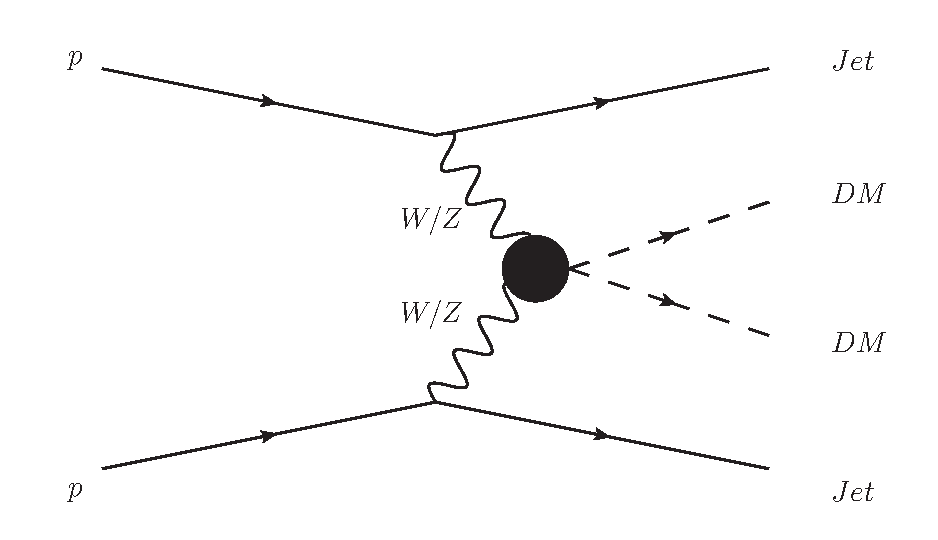
\includegraphics[width=7cm]{ppdmdmjj_feynman}
\end{column}
\begin{column}{.4\textwidth}
\begin{itemize}
\item Dimension BSM Operator and Tensor Structure
\item Dark Matter Mass
\item Mass of Mediating Particle (EFT Scale) 
\begin{itemize}
\item Affects the production rate ($\sigma$ scales with $\Lambda^{-2(D-4)}$)
\end{itemize}
\end{itemize}
\end{column}
\end{columns}
\end{frame}


\begin{frame}
\frametitle{Introduction to MadGraph Models}
\begin{itemize}
\item Models were originally discussed in Phys. Rev. D88 116009 (2013)
\item Had to start from scratch from the general lagrangian:
\end{itemize}
\center{( Mathematica $\to$ FeynRules ) $\to$ \textcolor{Plum}{\textbf{MadGraph}}}
\center{generate p p $\to$ chi chi j j}
\newline
\begin{itemize}
\item Pythia (Not using yet)
\item Rivet Analysis:
\begin{itemize}
\item Basic selection cuts
\item Kinematic distributions
\item Based on Atlas VBF Z/W + jets Analysis
\end{itemize}
\end{itemize}
\end{frame}

\begin{frame}
\frametitle{Outline of Different Operators}
\begin{columns}
\begin{column}{.3\textwidth} 
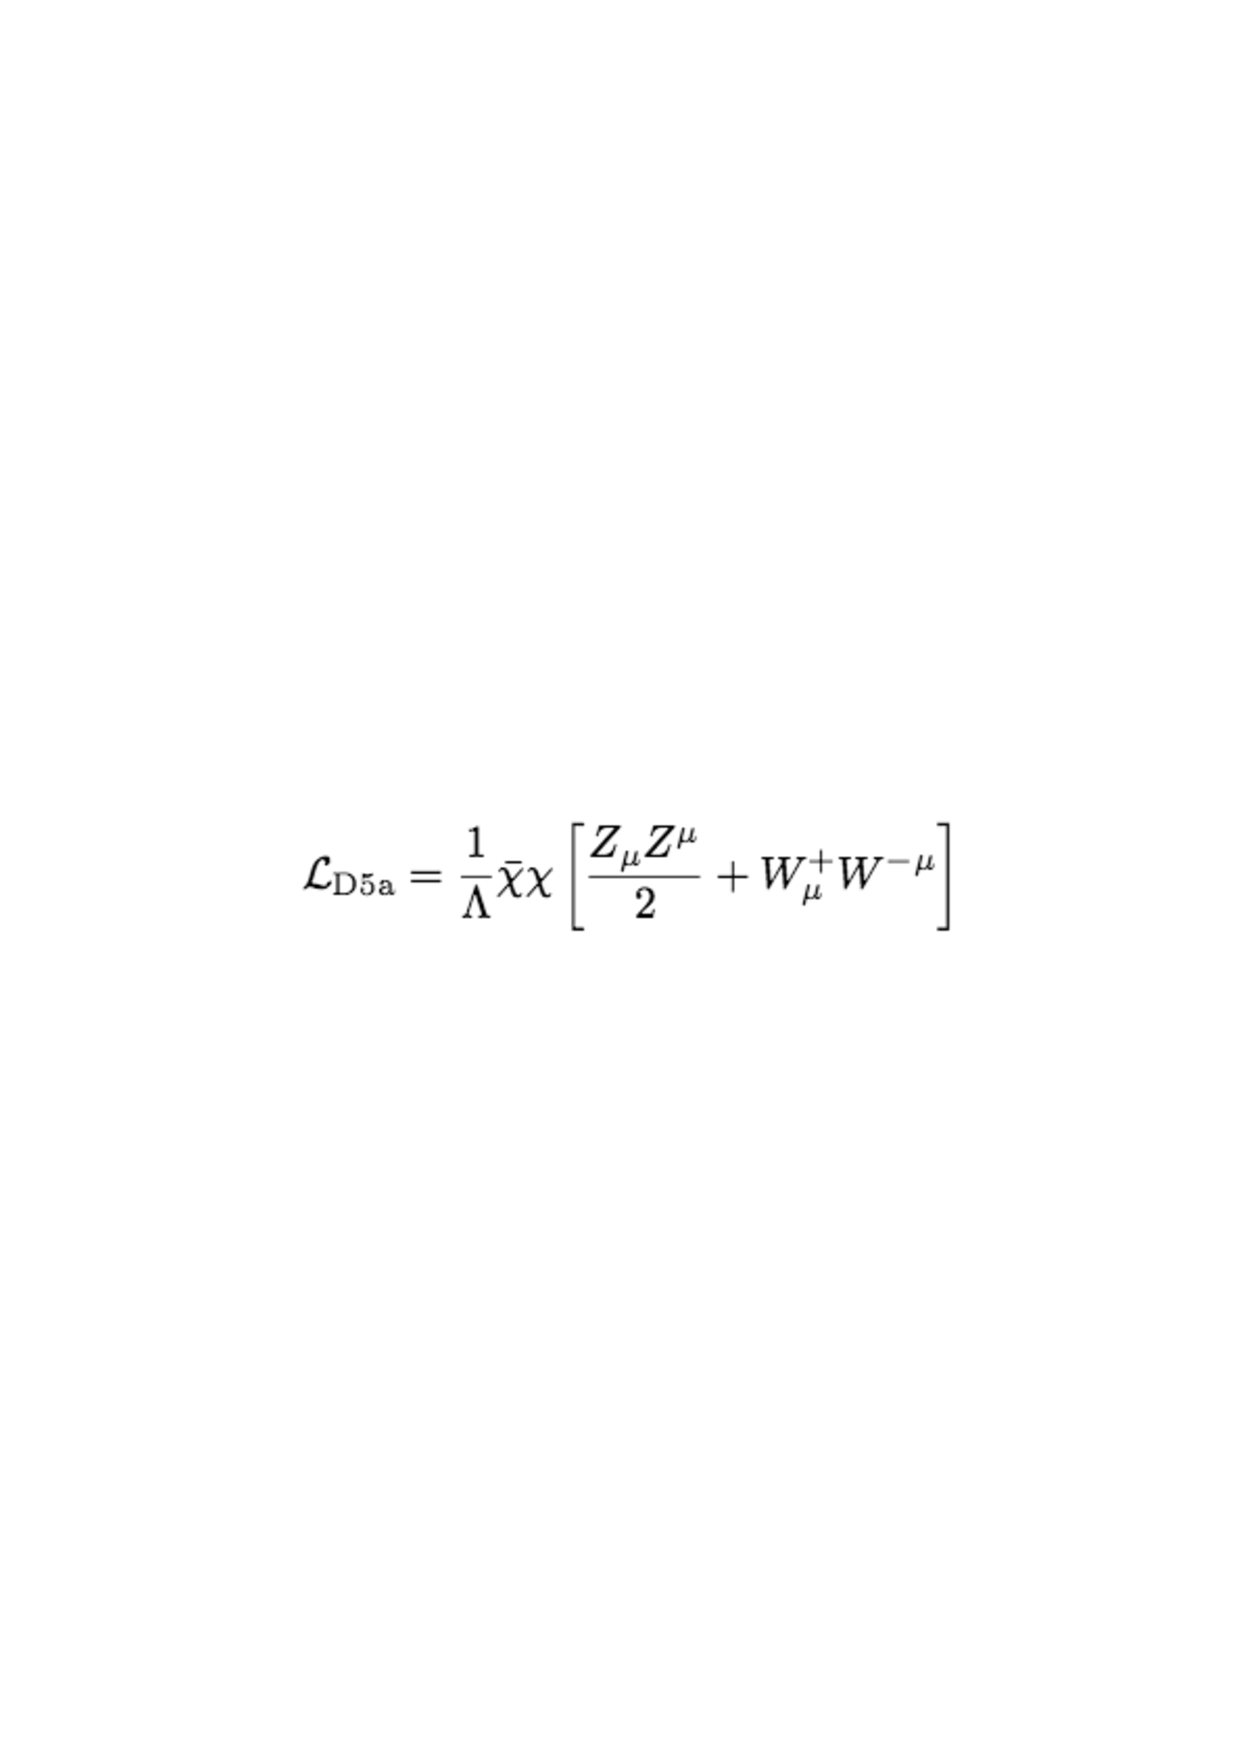
\includegraphics[width=4cm]{D5a_Lagrangian}
\newline \newline
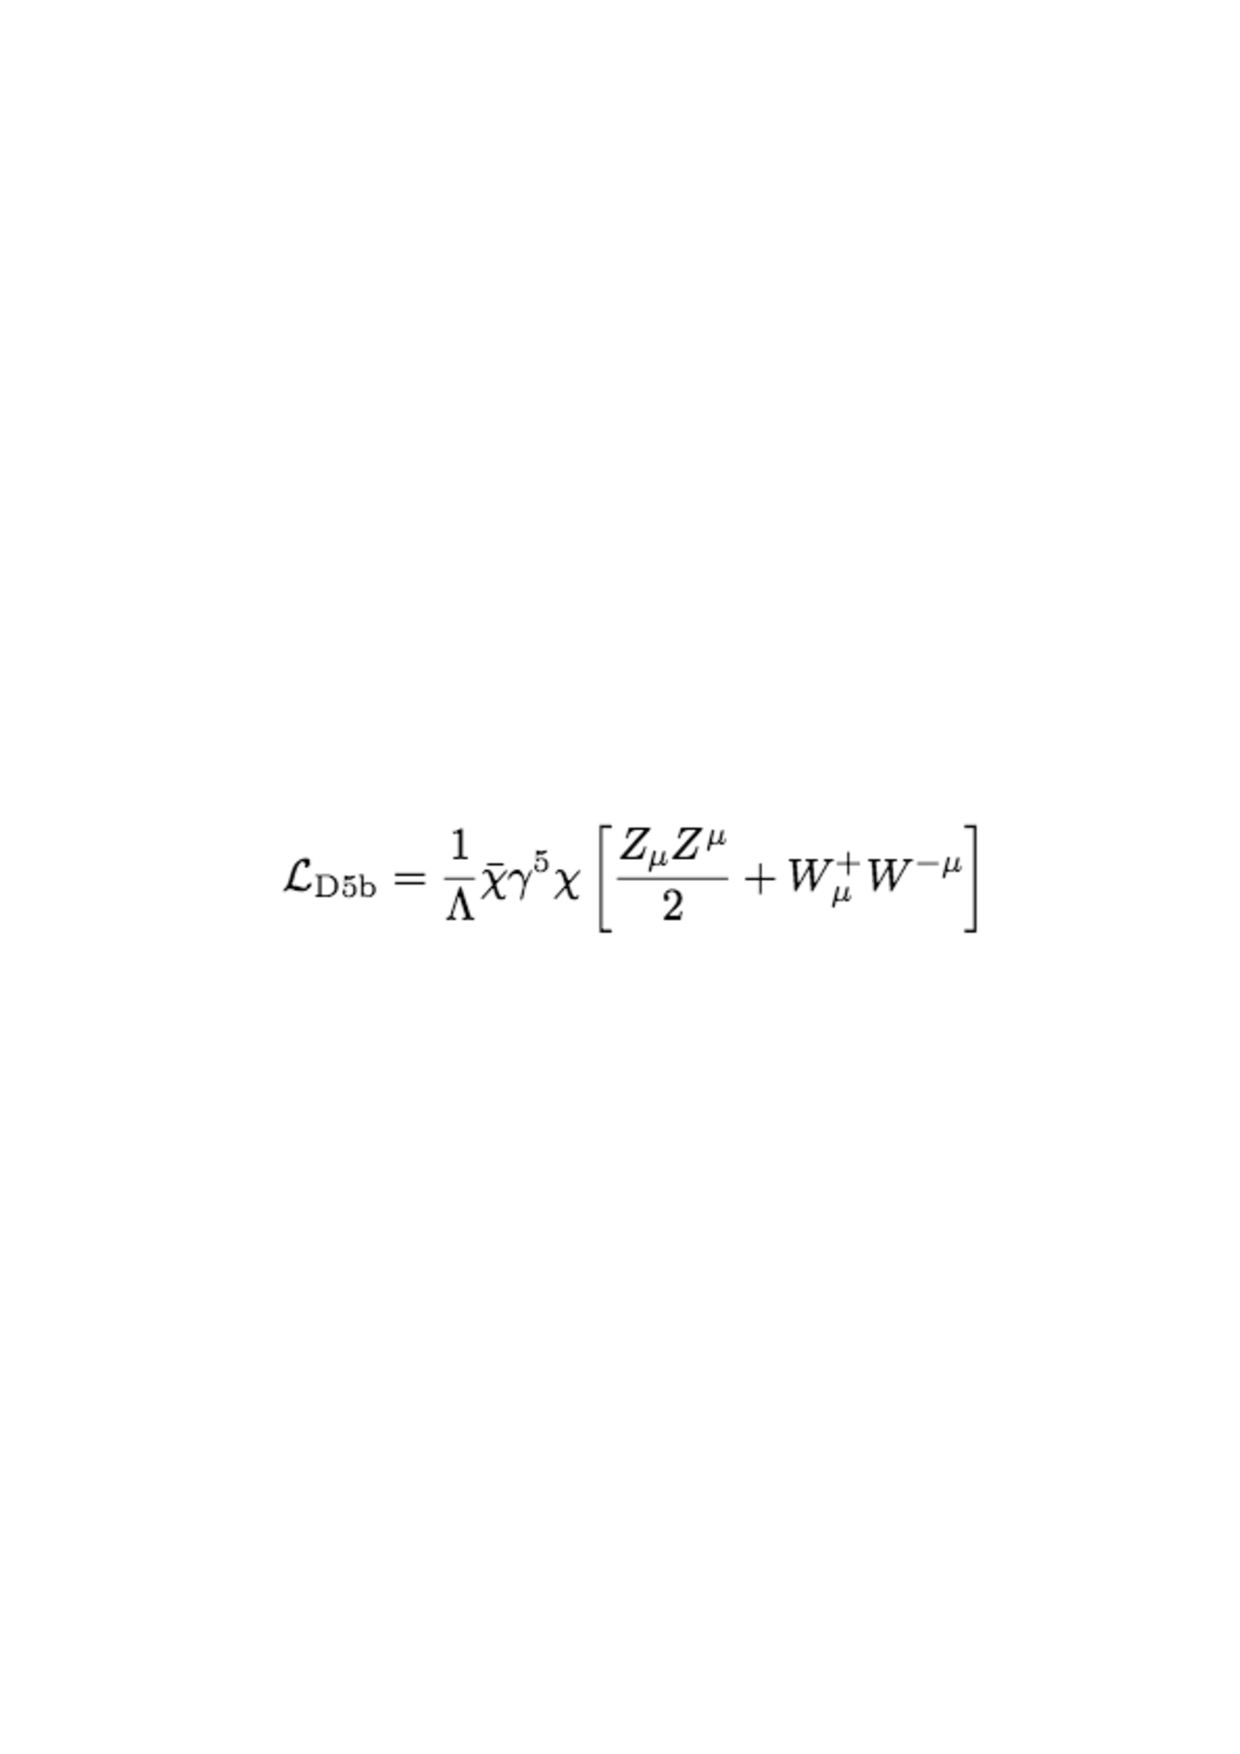
\includegraphics[width=4cm]{D5b_Lagrangian}
\newline \newline
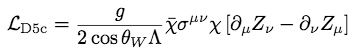
\includegraphics[width=4cm]{D5c_Lagrangian}
\end{column}
\begin{column}{.3\textwidth}
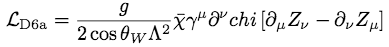
\includegraphics[width=4cm]{D6a_Lagrangian}
\newline \newline
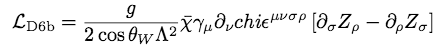
\includegraphics[width=4cm]{D6b_Lagrangian}
\newline \newline
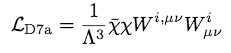
\includegraphics[width=4cm]{D7a_Lagrangian}
\end{column}
\begin{column}{.3\textwidth}
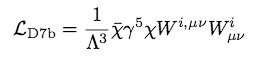
\includegraphics[width=4cm]{D7b_Lagrangian}
\newline \newline
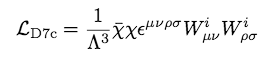
\includegraphics[width=4cm]{D7c_Lagrangian}
\newline \newline
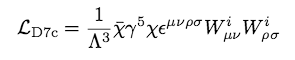
\includegraphics[width=4cm]{D7d_Lagrangian}
\end{column}
\end{columns}
\begin{itemize}
\item DM Mass and Lagrangian term influences the rates and kinematics.
\item Currently using baseline $\Lambda$ = 100GeV for all values, scaling as $\Lambda^{-2(D-4)}$.
\item Can study Higgs 'dark portal' where the interactions are the same as the BSM EFT:
\begin{itemize}
\item Plan to do so soon
\item Cross-check results with existing models in programs such as Sherpa.
\end{itemize}
\end{itemize}
\end{frame}



\begin{frame}
\frametitle{Phasespace Selection Cuts}
\textcolor{Plum}{\textbf{VBFZ Baseline:}} Jet1PT \textgreater 55 GeV; Jet2PT \textgreater 45 GeV; NumJets $\ge$ 2.
\newline
\newline \textcolor{Plum}{\textbf{VBFZ HighMass:}} Mjj \textgreater 1000 GeV; Jet1PT \textgreater 55 GeV; Jet2PT \textgreater 45 GeV; NumJets $\ge$ 2.
\newline
\newline \textcolor{Plum}{\textbf{VBFZ Search:}} Mjj \textgreater 250 GeV; Jet1PT \textgreater 55 GeV; Jet2PT \textgreater 45 GeV; NumJets $\ge$ 2. 
\begin{exampleblock}{\textcolor{Plum}{\textbf{VBFDM:}}}
Mjj \textgreater 250 GeV; Jet1PT \textgreater 55 GeV; Jet2PT \textgreater 45 GeV; NumJets $\ge$ 2; abseta \textless 4.4; MET \textgreater 150 GeV.
\end{exampleblock}
\textcolor{Plum}{\textbf{Monojet:}} Mjj \textgreater 250 GeV; Jet1PT \textgreater 45 GeV; NumJets $\ge$ 1; abseta \textless 4.4; MET \textgreater 150 GeV.
\newline
\newline \textcolor{Plum}{\textbf{VBFDM OR Monojet:}} VBFDM; Monojet.
\end{frame}

\begin{frame}
\frametitle{Distributions of interest:}
\begin{exampleblock}{Main distributions that have been produced:}
\begin{itemize}
\item Transverse Momentum of Jets, P$_{\text{T}}$(j1) and P$_{\text{T}}$(j2).
\item Dijet Mass, M$_{\text{jj}}$.
\item Missing Transverse Energy,  $\not{E}_{T}$.
\item Difference in Jet Angle $\Delta \phi$.
\item Difference in Jet Pseudorapidity, $\Delta \eta$.
\end{itemize}
\end{exampleblock}
\end{frame}

\begin{frame}
\frametitle{Distributions for D5a, VBFDM Selection, 10 GeV}
\begin{columns}
\begin{column}{.3\textwidth}
\center{DeltaEta}
\includegraphics[width=4cm]{/D5a/Mass10/MC_VBFDM_DeltaEta_PS_VBFDM.pdf}
\center{Mjj}
\includegraphics[width=4cm]{/D5a/Mass10/MC_VBFDM_Mjj_PS_VBFDM.pdf}
\end{column}
\begin{column}{.3\textwidth}
\center{DeltaPhi}
\includegraphics[width=4cm]{/D5a/Mass10/MC_VBFDM_DeltaPhi_PS_VBFDM.pdf}
\center{Jet1PT}
\includegraphics[width=4cm]{/D5a/Mass10/MC_VBFDM_Jet1PT_PS_VBFDM.pdf}
\end{column}
\begin{column}{.3\textwidth}
\center{ETMiss}
\includegraphics[width=4cm]{/D5a/Mass10/MC_VBFDM_ETMiss_PS_VBFDM.pdf}
\newline \newline \newline
Cross-section, $\sigma$ = 102 pb
\newline Acceptance = 26$\%$
\newline \newline \newline
\end{column}
\end{columns}
\begin{itemize}
\item DeltaPhi spectrum peaks
\end{itemize}
\end{frame}

\begin{frame}
\frametitle{Distributions for D5a, VBFDM Selection, 1000 GeV}
\begin{columns}
\begin{column}{.3\textwidth}
\center{DeltaEta}
\includegraphics[width=4cm]{/D5a/Mass1000/MC_VBFDM_DeltaEta_PS_VBFDM.pdf}
\center{Mjj}
\includegraphics[width=4cm]{/D5a/Mass1000/MC_VBFDM_Mjj_PS_VBFDM.pdf}
\end{column}
\begin{column}{.3\textwidth}
\center{DeltaPhi}
\includegraphics[width=4cm]{/D5a/Mass1000/MC_VBFDM_DeltaPhi_PS_VBFDM.pdf}
\center{Jet1PT}
\includegraphics[width=4cm]{/D5a/Mass1000/MC_VBFDM_Jet1PT_PS_VBFDM.pdf}
\end{column}
\begin{column}{.3\textwidth}
\center{ETMiss}
\includegraphics[width=4cm]{/D5a/Mass1000/MC_VBFDM_ETMiss_PS_VBFDM.pdf}
\newline \newline \newline
Cross-section, $\sigma$ = 9.1 pb
\newline Acceptance = 20$\%$
\newline \newline \newline
\end{column}
\end{columns}
\end{frame}

\begin{frame}
\frametitle{Distributions for D5b, VBFDM Selection, 10 GeV}
\begin{columns}
\begin{column}{.3\textwidth}
\center{DeltaEta}
\includegraphics[width=4cm]{/D5b/Mass10/MC_VBFDM_DeltaEta_PS_VBFDM.pdf}
\center{Mjj}
\includegraphics[width=4cm]{/D5b/Mass10/MC_VBFDM_Mjj_PS_VBFDM.pdf}
\end{column}
\begin{column}{.3\textwidth}
\center{DeltaPhi}
\includegraphics[width=4cm]{/D5b/Mass10/MC_VBFDM_DeltaPhi_PS_VBFDM.pdf}
\center{Jet1PT}
\includegraphics[width=4cm]{/D5b/Mass10/MC_VBFDM_Jet1PT_PS_VBFDM.pdf}
\end{column}
\begin{column}{.3\textwidth}
\center{ETMiss}
\includegraphics[width=4cm]{/D5b/Mass10/MC_VBFDM_ETMiss_PS_VBFDM.pdf}
\newline \newline \newline
Cross section, $\sigma$ = 102 pb
\newline Acceptance = 25$\%$
\newline \newline \newline
\end{column}
\end{columns}
\end{frame}

\begin{frame}
\frametitle{Distributions for D5b, VBFDM Selection, 1000 GeV}
\begin{columns}
\begin{column}{.3\textwidth}
\center{DeltaEta}
\includegraphics[width=4cm]{/D5b/Mass1000/MC_VBFDM_DeltaEta_PS_VBFDM.pdf}
\center{Mjj}
\includegraphics[width=4cm]{/D5b/Mass1000/MC_VBFDM_Mjj_PS_VBFDM.pdf}
\end{column}
\begin{column}{.3\textwidth}
\center{DeltaPhi}
\includegraphics[width=4cm]{/D5b/Mass1000/MC_VBFDM_DeltaPhi_PS_VBFDM.pdf}
\center{Jet1PT}
\includegraphics[width=4cm]{/D5b/Mass1000/MC_VBFDM_Jet1PT_PS_VBFDM.pdf}
\end{column}
\begin{column}{.3\textwidth}
\center{ETMiss}
\includegraphics[width=4cm]{/D5b/Mass1000/MC_VBFDM_ETMiss_PS_VBFDM.pdf}
\newline \newline \newline
Cross section, $\sigma$ = 18 pb
\newline Acceptance = 21$\%$
\newline \newline \newline
\end{column}
\end{columns}
\end{frame}

\begin{frame}
\frametitle{Distributions for D5c, VBFDM Selection, 10 GeV}
\begin{columns}
\begin{column}{.3\textwidth}
\center{DeltaEta}
\includegraphics[width=4cm]{/D5c/Mass10/MC_VBFDM_DeltaEta_PS_VBFDM.pdf}
\center{Mjj}
\includegraphics[width=4cm]{/D5c/Mass10/MC_VBFDM_Mjj_PS_VBFDM.pdf}
\end{column}
\begin{column}{.3\textwidth}
\center{DeltaPhi}
\includegraphics[width=4cm]{/D5c/Mass10/MC_VBFDM_DeltaPhi_PS_VBFDM.pdf}
\center{Jet1PT}
\includegraphics[width=4cm]{/D5c/Mass10/MC_VBFDM_Jet1PT_PS_VBFDM.pdf}
\end{column}
\begin{column}{.3\textwidth}
\center{ETMiss}
\includegraphics[width=4cm]{/D5c/Mass10/MC_VBFDM_ETMiss_PS_VBFDM.pdf}
\newline \newline \newline
Cross section, $\sigma$ = 4360 pb
\newline Acceptance = 4$\%$
\newline \newline \newline
\end{column}
\end{columns}
\begin{itemize}
\item The interaction would allow a new Z decay channel, which creates an invisible Z width constraint of $\Lambda$ \textgreater 3.3 TeV.
\end{itemize}
\end{frame}

\begin{frame}
\frametitle{Distributions for D5c, VBFDM Selection, 1000 GeV}
\begin{columns}
\begin{column}{.3\textwidth}
\center{DeltaEta}
\includegraphics[width=4cm]{/D5c/Mass1000/MC_VBFDM_DeltaEta_PS_VBFDM.pdf}
\center{Mjj}
\includegraphics[width=4cm]{/D5c/Mass1000/MC_VBFDM_Mjj_PS_VBFDM.pdf}
\end{column}
\begin{column}{.3\textwidth}
\center{DeltaPhi}
\includegraphics[width=4cm]{/D5c/Mass1000/MC_VBFDM_DeltaPhi_PS_VBFDM.pdf}
\center{Jet1PT}
\includegraphics[width=4cm]{/D5c/Mass1000/MC_VBFDM_Jet1PT_PS_VBFDM.pdf}
\end{column}
\begin{column}{.3\textwidth}
\center{ETMiss}
\includegraphics[width=4cm]{/D5c/Mass1000/MC_VBFDM_ETMiss_PS_VBFDM.pdf}
\newline \newline \newline
Cross section, $\sigma$ = 37 pb
\newline Acceptance = 42$\%$
\newline \newline \newline
\end{column}
\end{columns}
\begin{itemize}
\item Invisible Z width constraint of $\Lambda$ \textgreater 6.6 TeV. This gives a very high suppression factor: 4.5x10$^{3}$.
\end{itemize}
\end{frame}

\begin{frame}
\frametitle{Distributions for D6a, VBFDM Selection, 10 GeV}
\begin{columns}
\begin{column}{.3\textwidth}
\center{DeltaEta}
\includegraphics[width=4cm]{/D6a/Mass10/MC_VBFDM_DeltaEta_PS_VBFDM.pdf}
\center{Mjj}
\includegraphics[width=4cm]{/D6a/Mass10/MC_VBFDM_Mjj_PS_VBFDM.pdf}
\end{column}
\begin{column}{.3\textwidth}
\center{DeltaPhi}
\includegraphics[width=4cm]{/D6a/Mass10/MC_VBFDM_DeltaPhi_PS_VBFDM.pdf}
\center{Jet1PT}
\includegraphics[width=4cm]{/D6a/Mass10/MC_VBFDM_Jet1PT_PS_VBFDM.pdf}
\end{column}
\begin{column}{.3\textwidth}
\center{ETMiss}
\includegraphics[width=4cm]{/D6a/Mass10/MC_VBFDM_ETMiss_PS_VBFDM.pdf}
\newline \newline \newline
Cross section, $\sigma$ = 151 pb
\newline Acceptance = 11$\%$
\newline \newline \newline
\end{column}
\end{columns}
\begin{itemize}
\item Invisible Z width constraint of $\Lambda$ \textgreater 230GeV. This gives a very high suppression factor: 30.
\end{itemize}
\end{frame}

\begin{frame}
\frametitle{Distributions for D6a, VBFDM Selection, 1000 GeV}
\begin{columns}
\begin{column}{.3\textwidth}
\center{DeltaEta}
\includegraphics[width=4cm]{/D6a/Mass1000/MC_VBFDM_DeltaEta_PS_VBFDM.pdf}
\center{Mjj}
\includegraphics[width=4cm]{/D6a/Mass1000/MC_VBFDM_Mjj_PS_VBFDM.pdf}
\end{column}
\begin{column}{.3\textwidth}
\center{DeltaPhi}
\includegraphics[width=4cm]{/D6a/Mass1000/MC_VBFDM_DeltaPhi_PS_VBFDM.pdf}
\center{Jet1PT}
\includegraphics[width=4cm]{/D6a/Mass1000/MC_VBFDM_Jet1PT_PS_VBFDM.pdf}
\end{column}
\begin{column}{.3\textwidth}
\center{ETMiss}
\includegraphics[width=4cm]{/D6a/Mass1000/MC_VBFDM_ETMiss_PS_VBFDM.pdf}
\newline \newline \newline
Cross section, $\sigma$ = 4.96 pb
\newline Acceptance = 42$\%$
\newline \newline \newline
\end{column}
\end{columns}
\begin{itemize}
\item DeltaEta distribution is quite low.
\item DeltaPhi distribution is flat compared to the rest.
\end{itemize}
\end{frame}

\begin{frame}
\frametitle{Distributions for D6b, VBFDM Selection, 10 GeV}
\begin{columns}
\begin{column}{.3\textwidth}
\center{DeltaEta}
\includegraphics[width=4cm]{/D6b/Mass10/MC_VBFDM_DeltaEta_PS_VBFDM.pdf}
\center{Mjj}
\includegraphics[width=4cm]{/D6b/Mass10/MC_VBFDM_Mjj_PS_VBFDM.pdf}
\end{column}
\begin{column}{.3\textwidth}
\center{DeltaPhi}
\includegraphics[width=4cm]{/D6b/Mass10/MC_VBFDM_DeltaPhi_PS_VBFDM.pdf}
\center{Jet1PT}
\includegraphics[width=4cm]{/D6b/Mass10/MC_VBFDM_Jet1PT_PS_VBFDM.pdf}
\end{column}
\begin{column}{.3\textwidth}
\center{ETMiss}
\includegraphics[width=4cm]{/D6b/Mass10/MC_VBFDM_ETMiss_PS_VBFDM.pdf}
\newline \newline \newline
Cross section, $\sigma$ = 562 pb
\newline Acceptance = 13$\%$
\newline \newline \newline
\end{column}
\end{columns}
\begin{itemize}
\item Invisible Z width constraint of $\Lambda$ \textgreater 330GeV. This gives a very high suppression factor: 120.
\end{itemize}
\end{frame}

\begin{frame}
\frametitle{Distributions for D6b, VBFDM Selection, 1000 GeV}
\begin{columns}
\begin{column}{.3\textwidth}
\center{DeltaEta}
\includegraphics[width=4cm]{/D6b/Mass1000/MC_VBFDM_DeltaEta_PS_VBFDM.pdf}
\center{Mjj}
\includegraphics[width=4cm]{/D6b/Mass1000/MC_VBFDM_Mjj_PS_VBFDM.pdf}
\end{column}
\begin{column}{.3\textwidth}
\center{DeltaPhi}
\includegraphics[width=4cm]{/D6b/Mass1000/MC_VBFDM_DeltaPhi_PS_VBFDM.pdf}
\center{Jet1PT}
\includegraphics[width=4cm]{/D6b/Mass1000/MC_VBFDM_Jet1PT_PS_VBFDM.pdf}
\end{column}
\begin{column}{.3\textwidth}
\center{ETMiss}
\includegraphics[width=4cm]{/D6b/Mass1000/MC_VBFDM_ETMiss_PS_VBFDM.pdf}
\newline \newline \newline
Cross section, $\sigma$ = 4.2 pb
\newline Acceptance = 42$\%$
\newline \newline \newline
\end{column}
\end{columns}
\begin{itemize}
\item Very flat Jet P$_{\text{T}}$ spectrum.
\end{itemize}
\end{frame}

\begin{frame}
\frametitle{Distributions for D7a, VBFDM Selection, 10 GeV}
\begin{columns}
\begin{column}{.3\textwidth}
\center{DeltaEta}
\includegraphics[width=4cm]{/D7a/Mass10/MC_VBFDM_DeltaEta_PS_VBFDM.pdf}
\center{Mjj}
\includegraphics[width=4cm]{/D7a/Mass10/MC_VBFDM_Mjj_PS_VBFDM.pdf}
\end{column}
\begin{column}{.3\textwidth}
\center{DeltaPhi}
\includegraphics[width=4cm]{/D7a/Mass10/MC_VBFDM_DeltaPhi_PS_VBFDM.pdf}
\center{Jet1PT}
\includegraphics[width=4cm]{/D7a/Mass10/MC_VBFDM_Jet1PT_PS_VBFDM.pdf}
\end{column}
\begin{column}{.3\textwidth}
\center{ETMiss}
\includegraphics[width=4cm]{/D7a/Mass10/MC_VBFDM_ETMiss_PS_VBFDM.pdf}
\newline \newline \newline
Cross section, $\sigma$ = 4240 pb
\newline Acceptance = 78$\%$
\newline \newline \newline
\end{column}
\end{columns}
\begin{itemize}
\item DeltaEta distribution is very broad.
\item Perhaps some modulation in DeltaPhi?
\end{itemize}
\end{frame}

\begin{frame}
\frametitle{Distributions for D7a, VBFDM Selection, 1000 GeV}
\begin{columns}
\begin{column}{.3\textwidth}
\center{DeltaEta}
\includegraphics[width=4cm]{/D7a/Mass1000/MC_VBFDM_DeltaEta_PS_VBFDM.pdf}
\center{Mjj}
\includegraphics[width=4cm]{/D7a/Mass1000/MC_VBFDM_Mjj_PS_VBFDM.pdf}
\end{column}
\begin{column}{.3\textwidth}
\center{DeltaPhi}
\includegraphics[width=4cm]{/D7a/Mass1000/MC_VBFDM_DeltaPhi_PS_VBFDM.pdf}
\center{Jet1PT}
\includegraphics[width=4cm]{/D7a/Mass1000/MC_VBFDM_Jet1PT_PS_VBFDM.pdf}
\end{column}
\begin{column}{.3\textwidth}
\center{ETMiss}
\includegraphics[width=4cm]{/D7a/Mass1000/MC_VBFDM_ETMiss_PS_VBFDM.pdf}
\newline \newline \newline
Cross section, $\sigma$ = 10200 pb
\newline Acceptance = 75$\%$
\newline \newline \newline
\end{column}
\end{columns}
\end{frame}

\begin{frame}
\frametitle{Distributions for D7b, VBFDM Selection, 10 GeV}
\begin{columns}
\begin{column}{.3\textwidth}
\center{DeltaEta}
\includegraphics[width=4cm]{/D7b/Mass10/MC_VBFDM_DeltaEta_PS_VBFDM.pdf}
\center{Mjj}
\includegraphics[width=4cm]{/D7b/Mass10/MC_VBFDM_Mjj_PS_VBFDM.pdf}
\end{column}
\begin{column}{.3\textwidth}
\center{DeltaPhi}
\includegraphics[width=4cm]{/D7b/Mass10/MC_VBFDM_DeltaPhi_PS_VBFDM.pdf}
\center{Jet1PT}
\includegraphics[width=4cm]{/D7b/Mass10/MC_VBFDM_Jet1PT_PS_VBFDM.pdf}
\end{column}
\begin{column}{.3\textwidth}
\center{ETMiss}
\includegraphics[width=4cm]{/D7b/Mass10/MC_VBFDM_ETMiss_PS_VBFDM.pdf}
\newline \newline \newline
Cross section, $\sigma$ = 41900 pb
\newline Acceptance = 78$\%$
\newline \newline \newline
\end{column}
\end{columns}
\end{frame}

\begin{frame}
\frametitle{Distributions for D7b, VBFDM Selection, 1000 GeV}
\begin{columns}
\begin{column}{.3\textwidth}
\center{DeltaEta}
\includegraphics[width=4cm]{/D7b/Mass1000/MC_VBFDM_DeltaEta_PS_VBFDM.pdf}
\center{Mjj}
\includegraphics[width=4cm]{/D7b/Mass1000/MC_VBFDM_Mjj_PS_VBFDM.pdf}
\end{column}
\begin{column}{.3\textwidth}
\center{DeltaPhi}
\includegraphics[width=4cm]{/D7b/Mass1000/MC_VBFDM_DeltaPhi_PS_VBFDM.pdf}
\center{Jet1PT}
\includegraphics[width=4cm]{/D7b/Mass1000/MC_VBFDM_Jet1PT_PS_VBFDM.pdf}
\end{column}
\begin{column}{.3\textwidth}
\center{ETMiss}
\includegraphics[width=4cm]{/D7b/Mass1000/MC_VBFDM_ETMiss_PS_VBFDM.pdf}
\newline \newline \newline
Cross section, $\sigma$ = 17600 pb
\newline Acceptance = 76$\%$
\newline \newline \newline
\end{column}
\end{columns}
\end{frame}

\begin{frame}
\frametitle{Distributions for D7c, VBFDM Selection, 10 GeV}
\begin{columns}
\begin{column}{.3\textwidth}
\center{DeltaEta}
\includegraphics[width=4cm]{/D7c/Mass10/MC_VBFDM_DeltaEta_PS_VBFDM.pdf}
\center{Mjj}
\includegraphics[width=4cm]{/D7c/Mass10/MC_VBFDM_Mjj_PS_VBFDM.pdf}
\end{column}
\begin{column}{.3\textwidth}
\center{DeltaPhi}
\includegraphics[width=4cm]{/D7c/Mass10/MC_VBFDM_DeltaPhi_PS_VBFDM.pdf}
\center{Jet1PT}
\includegraphics[width=4cm]{/D7c/Mass10/MC_VBFDM_Jet1PT_PS_VBFDM.pdf}
\end{column}
\begin{column}{.3\textwidth}
\center{ETMiss}
\includegraphics[width=4cm]{/D7c/Mass10/MC_VBFDM_ETMiss_PS_VBFDM.pdf}
\newline \newline \newline
Cross section, $\sigma$ = 167000 pb
\newline Acceptance = 80$\%$
\newline \newline \newline
\end{column}
\end{columns}
\end{frame}

\begin{frame}
\frametitle{Distributions for D7c, VBFDM Selection, 1000 GeV}
\begin{columns}
\begin{column}{.3\textwidth}
\center{DeltaEta}
\includegraphics[width=4cm]{/D7c/Mass1000/MC_VBFDM_DeltaEta_PS_VBFDM.pdf}
\center{Mjj}
\includegraphics[width=4cm]{/D7c/Mass1000/MC_VBFDM_Mjj_PS_VBFDM.pdf}
\end{column}
\begin{column}{.3\textwidth}
\center{DeltaPhi}
\includegraphics[width=4cm]{/D7c/Mass1000/MC_VBFDM_DeltaPhi_PS_VBFDM.pdf}
\center{Jet1PT}
\includegraphics[width=4cm]{/D7c/Mass1000/MC_VBFDM_Jet1PT_PS_VBFDM.pdf}
\end{column}
\begin{column}{.3\textwidth}
\center{ETMiss}
\includegraphics[width=4cm]{/D7c/Mass1000/MC_VBFDM_ETMiss_PS_VBFDM.pdf}
\newline \newline \newline
Cross section, $\sigma$ = 40900 pb
\newline Acceptance = 78$\%$
\newline \newline \newline
\end{column}
\end{columns}
\end{frame}

\begin{frame}
\frametitle{Distributions for D7d, VBFDM Selection, 10 GeV}
\begin{columns}
\begin{column}{.3\textwidth}
\center{DeltaEta}
\includegraphics[width=4cm]{/D7d/Mass10/MC_VBFDM_DeltaEta_PS_VBFDM.pdf}
\center{Mjj}
\includegraphics[width=4cm]{/D7d/Mass10/MC_VBFDM_Mjj_PS_VBFDM.pdf}
\end{column}
\begin{column}{.3\textwidth}
\center{DeltaPhi}
\includegraphics[width=4cm]{/D7d/Mass10/MC_VBFDM_DeltaPhi_PS_VBFDM.pdf}
\center{Jet1PT}
\includegraphics[width=4cm]{/D7d/Mass10/MC_VBFDM_Jet1PT_PS_VBFDM.pdf}
\end{column}
\begin{column}{.3\textwidth}
\center{ETMiss}
\includegraphics[width=4cm]{/D7d/Mass10/MC_VBFDM_ETMiss_PS_VBFDM.pdf}
\newline \newline \newline
Cross section, $\sigma$ = 168000 pb
\newline Acceptance = 79$\%$
\newline \newline \newline
\end{column}
\end{columns}
\begin{itemize}
\item DeltaPhi again has different structure.
\end{itemize}
\end{frame}

\begin{frame}
\frametitle{Distributions for D7d, VBFDM Selection, 1000 GeV}
\begin{columns}
\begin{column}{.3\textwidth}
\center{DeltaEta}
\includegraphics[width=4cm]{/D7d/Mass1000/MC_VBFDM_DeltaEta_PS_VBFDM.pdf}
\center{Mjj}
\includegraphics[width=4cm]{/D7d/Mass1000/MC_VBFDM_Mjj_PS_VBFDM.pdf}
\end{column}
\begin{column}{.3\textwidth}
\center{DeltaPhi}
\includegraphics[width=4cm]{/D7d/Mass1000/MC_VBFDM_DeltaPhi_PS_VBFDM.pdf}
\center{Jet1PT}
\includegraphics[width=4cm]{/D7d/Mass1000/MC_VBFDM_Jet1PT_PS_VBFDM.pdf}
\end{column}
\begin{column}{.3\textwidth}
\center{ETMiss}
\includegraphics[width=4cm]{/D7d/Mass1000/MC_VBFDM_ETMiss_PS_VBFDM.pdf}
\newline \newline \newline
Cross section, $\sigma$ = 68800 pb
\newline Acceptance = 78$\%$
\newline \newline \newline
\end{column}
\end{columns}
\end{frame}

\begin{frame}
\frametitle{Next Steps:}
\begin{itemize}
\item Overlays of distributions for various operators/masses.
\item Automation of current run through, as well as looking at:
\begin{itemize}
\item Any other distributions of interest.
\item Any other phase spaces (Any gains from relaxed requirements?)
\item Scan all mass/dimension parameter space.
\end{itemize}
\item Look at invisible Higgs validation of Sherpa.
\item Add three jet contributions later.
\item Indicative simulated sample through Atlas production system.
\item Check regions of differential distributions for EFT validity.
\item Run through Rivet routine with background processes to compare to signal kinematics. \newline Mainly SM( Z $\to$ $\nu$ $\bar{\nu}$ ) + j j.
\item Any other thoughts?
\end{itemize}
\end{frame}







\end{document} 